% Source: graduate-coursework/Research/Intro_to_Agents/handouts/Part7_Parallelization.tex

\documentclass[border=4pt]{standalone}
\usepackage{amsmath,amssymb,amsfonts}
\usepackage[T1]{fontenc}
\usepackage{graphicx}
\usepackage{lmodern}
\usepackage{tikz}
\usepackage{xcolor}
\usetikzlibrary{shapes.geometric, arrows.meta, positioning, calc, fit, backgrounds, matrix, decorations.pathreplacing}

\definecolor{UofSCGarnet}{HTML}{73000a}
\definecolor{UofSCBlack}{HTML}{000000}
\definecolor{UofSCWhite}{HTML}{ffffff}
\definecolor{UofSCRose}{HTML}{CC2E40}
\definecolor{UofSCAtlantic}{HTML}{466A9F}
\definecolor{UofSCCongaree}{HTML}{1F414D}
\definecolor{UofSCHorseshoe}{HTML}{65780B}
\definecolor{UofSCGrass}{HTML}{CED318}
\definecolor{UofSCHoneycomb}{HTML}{A49137}
\definecolor{UofSC90Black}{HTML}{363636}
\definecolor{UofSC70Black}{HTML}{5C5C5C}
\definecolor{UofSC50Black}{HTML}{A2A2A2}
\definecolor{UofSCWarmGrey}{HTML}{676156}
\definecolor{UofSCSandstorm}{HTML}{FFF2E3}
\definecolor{UofSCDarkGarnet}{HTML}{570008}
\definecolor{UofSCAzalea}{HTML}{844247}

\tikzset{
    % Node styles - all with sharp corners
    agentbox/.style={
        rectangle,
        draw=UofSCGarnet,
        fill=UofSCSandstorm,
        thick,
        minimum width=2cm,
        minimum height=0.8cm,
        text centered,
        font=\footnotesize
    },
    processbox/.style={
        rectangle,
        draw=UofSCAtlantic,
        fill=UofSCWhite,
        thick,
        minimum width=2.5cm,
        minimum height=0.7cm,
        text centered,
        font=\footnotesize
    },
    syncbox/.style={
        rectangle,
        draw=UofSCCongaree,
        fill=UofSCCongaree!20,
        thick,
        minimum width=3cm,
        minimum height=0.5cm,
        text centered,
        font=\footnotesize\bfseries
    },
    resultbox/.style={
        rectangle,
        draw=UofSCHorseshoe,
        fill=UofSCGrass!30,
        thick,
        minimum width=2cm,
        minimum height=0.7cm,
        text centered,
        font=\footnotesize
    },
    % Arrow styles
    myarrow/.style={
        ->,
        >=Stealth,
        thick,
        UofSCBlack
    },
    dashedarrow/.style={
        ->,
        >=Stealth,
        thick,
        dashed,
        UofSC70Black
    },
    % Timeline styles
    timeline/.style={
        draw=UofSCBlack,
        thick,
        ->,
        >=Stealth
    },
    timeblock/.style={
        rectangle,
        draw=none,
        minimum height=0.5cm,
        text centered,
        font=\tiny
    }
}

\begin{document}
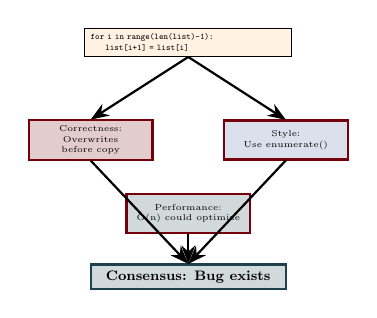
\begin{tikzpicture}[scale=0.62, transform shape]
                % Code snippet
                \node[rectangle,draw=UofSCBlack,fill=UofSCSandstorm,text width=4cm,font=\tiny\ttfamily] (code) at (2,4.5) {
                    for i in range(len(list)-1):\\
                    \hspace{0.3cm}list[i+1] = list[i]
                };

                % Three reviewers
                \node[agentbox,fill=UofSCGarnet!20,minimum width=2.5cm,text width=2.3cm,font=\tiny] (r1) at (0,2.5) {Correctness:\\Overwrites before copy};
                \node[agentbox,fill=UofSCAtlantic!20,minimum width=2.5cm,text width=2.3cm,font=\tiny] (r2) at (4,2.5) {Style:\\Use enumerate()};
                \node[agentbox,fill=UofSCCongaree!20,minimum width=2.5cm,text width=2.3cm,font=\tiny] (r3) at (2,1) {Performance:\\O(n) could optimize};

                % Consensus
                \node[syncbox,minimum width=4cm] (cons) at (2,-0.3) {Consensus: Bug exists};

                % Arrows
                \draw[myarrow] (code.south) -- (r1.north);
                \draw[myarrow] (code.south) -- (r2.north);
                \draw[myarrow] (r1.south) -- (cons.north);
                \draw[myarrow] (r2.south) -- (cons.north);
                \draw[myarrow] (r3.south) -- (cons.north);
            \end{tikzpicture}
\end{document}
